Firstly the ROI is found. 

There are several approaches that could be used:
\begin{itemize}
	\item Search for the table as a big rectangle.
	\item Searching for the holes on the pool table.
	\item Finding the most common colour (the cloth) and then find the outer points of the cloth.
\end{itemize}

A combination of the first and last approach is used.

The method used is explained by this flowchart\ref{fig:detecttable_flowchart}:

\begin{figure}[H]
\begin{center}
\leavevmode
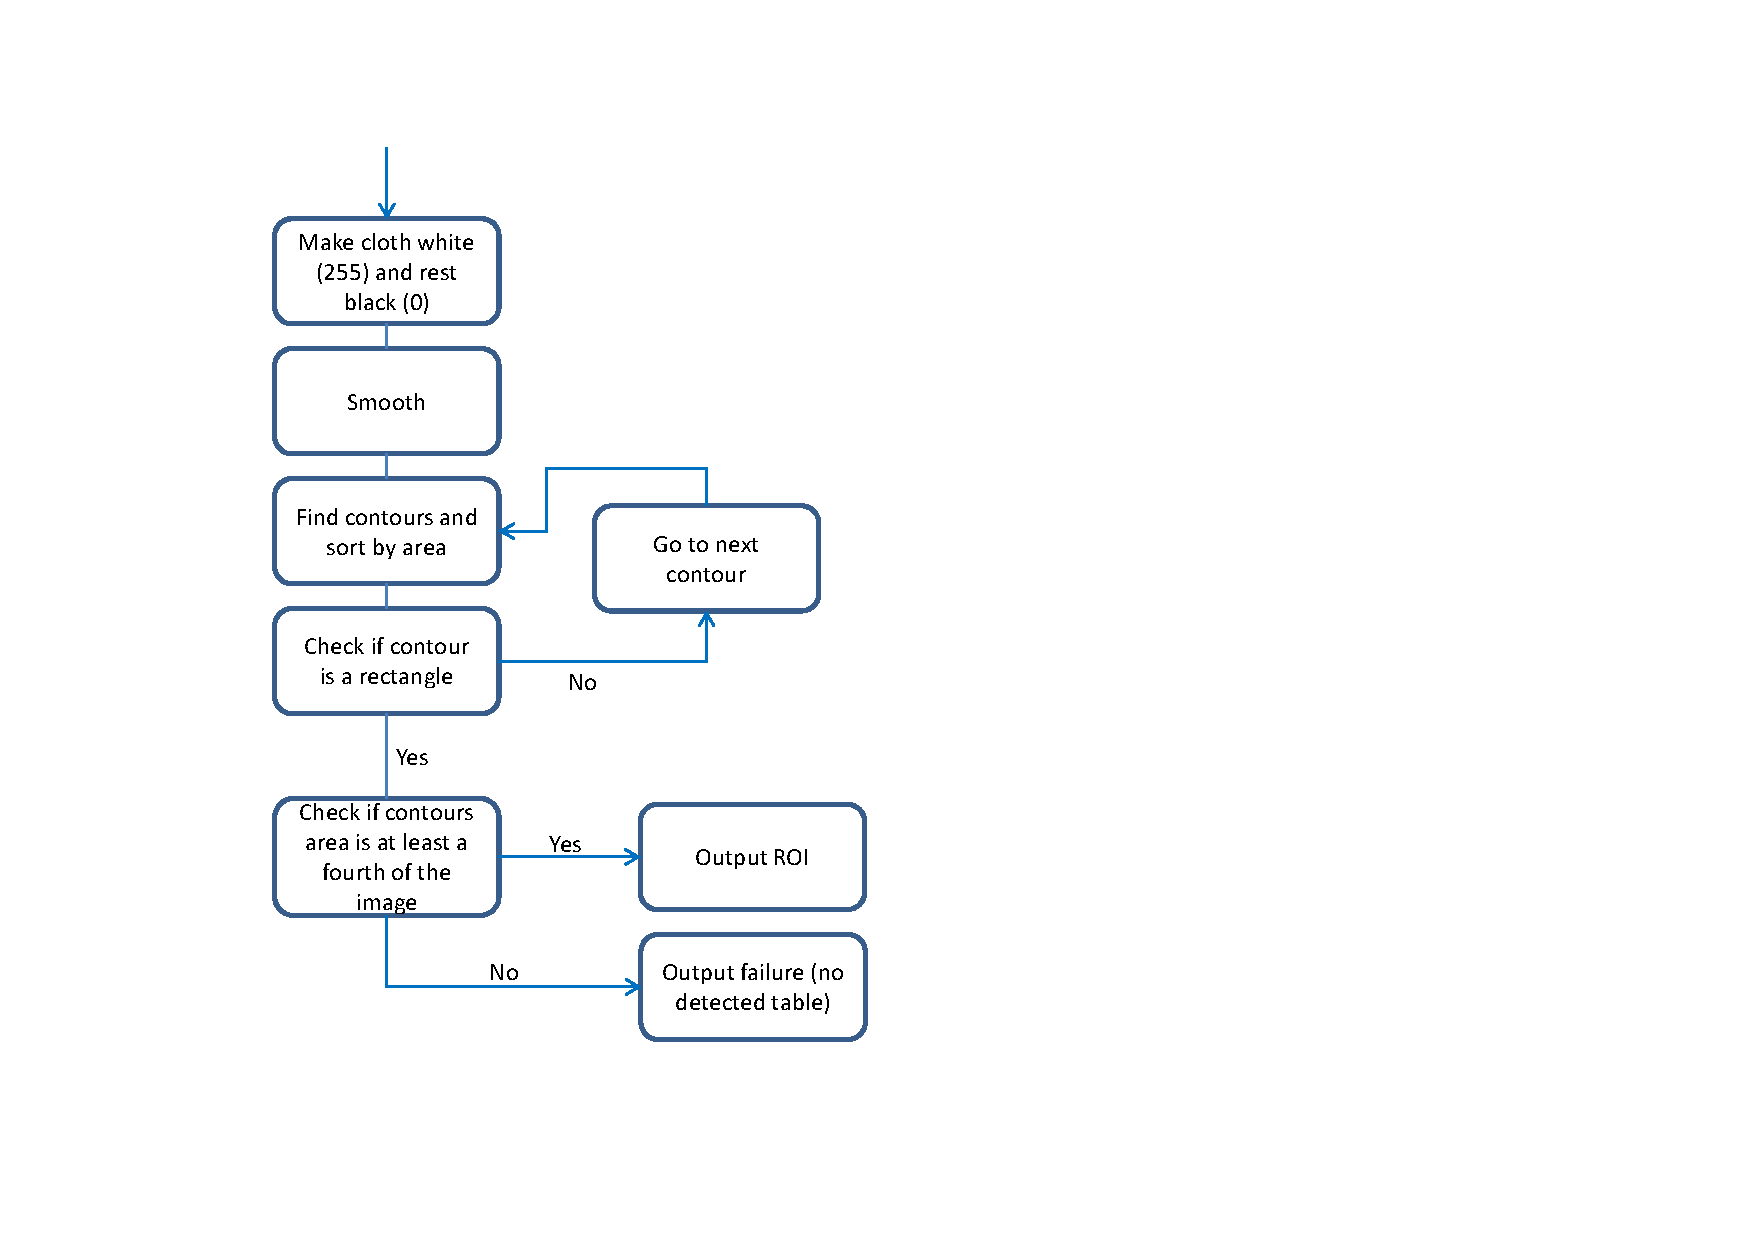
\includegraphics[width=0.5\textwidth]{images/tabledetect_flowchat.pdf}
\end{center}
\caption{Flowchart explaining table detection.}
\label{fig:detecttable_flowchart}
\end{figure}

The following steps will be done:
\begin{enumerate}
\item Using the method explained in \ref{sec:removeback} will provide an image where the cloth has been removed. Instead of removing the cloth the returned image will consists of white pixels where the cloth is and black where it was not found. This will be as this image:

%INSERT IMAGE WITHOUT CLOTH.

\item The image is now smoothed using a gaussian kernel which will decrease the noise.

\item Find the contours of the image by using chain code as explained in \ref{sec:contours}. When found the contours are sorted by area.

\item Check if the contour is a rectangle. This i done by converting the vertices of the contour into lines. These lines should lie orthogonal to each other or a lest very close to.

By measuring the angle between the intersecting lines and check whether they lie in a selected interval [85\degree;95\degree], it can be determined if the contour is a well defined rectangle which a pool table is.

If some of the lines angle are not in the selected interval the contour will be discarded and step 4 will be repeated for the next contour.

\item The pool table has to take up at least 25\% of the image. If a contour is found to be rectangular, but does not take up at least this percentage the algorithm will not return a ROI (region of interest). If the contour is larger or 25\% the contour is considered to be the pool table and the ROI will be returned.
\end{enumerate}